%!TEX root=presentation.tex

\section{Inledning}


\begin{frame}
\frametitle{Cutkoskys handmodeller}
\includegraphics[width=0.85\textwidth]{img/cutkoskys_handmodeller}
\end{frame}

\begin{frame}
\frametitle{Cutkoskys handmodeller}
\includegraphics[width=0.85\textwidth]{img/cutkoskyscadgrepp}
\end{frame}


\begin{frame}
\begin{columns}
\begin{column}{0.5\textwidth}
\includegraphics[height=0.45\textheight]{img/milk}

\includegraphics[height=0.45\textheight]{img/snusgrepp}
\end{column}

\begin{column}{0.5\textwidth}
\includegraphics[height=0.45\textheight]{img/mutterlyft}

\includegraphics[height=0.4\textheight]{img/cylinder}
\end{column}
\end{columns}
\end{frame}

\begin{frame}
\frametitle{Flödesschema}
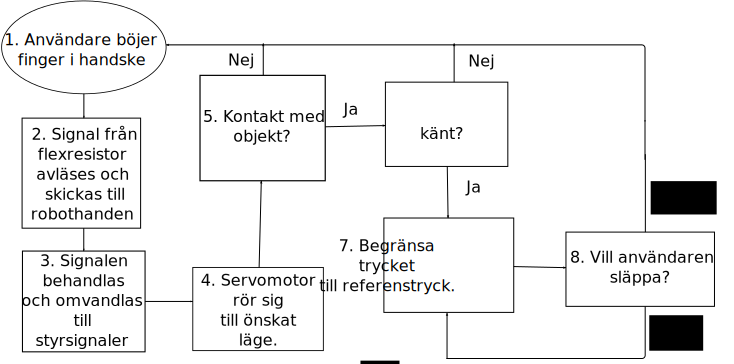
\includegraphics[width=\textwidth]{img/flodesschema}
\end{frame}

\section{Robothanden}
\begin{frame}
\frametitle{Robothand}
\includegraphics[width=\textwidth]{img/hand}
\end{frame}
\begin{frame}
\frametitle{Finger}
\includegraphics[width=\textwidth]{img/fingerbild}
\end{frame}
\begin{frame}
\frametitle{Stag och sena}
\includegraphics[width=\textwidth]{img/stagsenor}
\end{frame}
\begin{frame}
\frametitle{Fingertoppar}
\includegraphics[width=0.5\textwidth]{img/sensor}
\includegraphics[width=0.55\textwidth]{img/trycksensor}
\end{frame}

\section{Styrhandsken}
\begin{frame}
\frametitle{Styrhandsken}
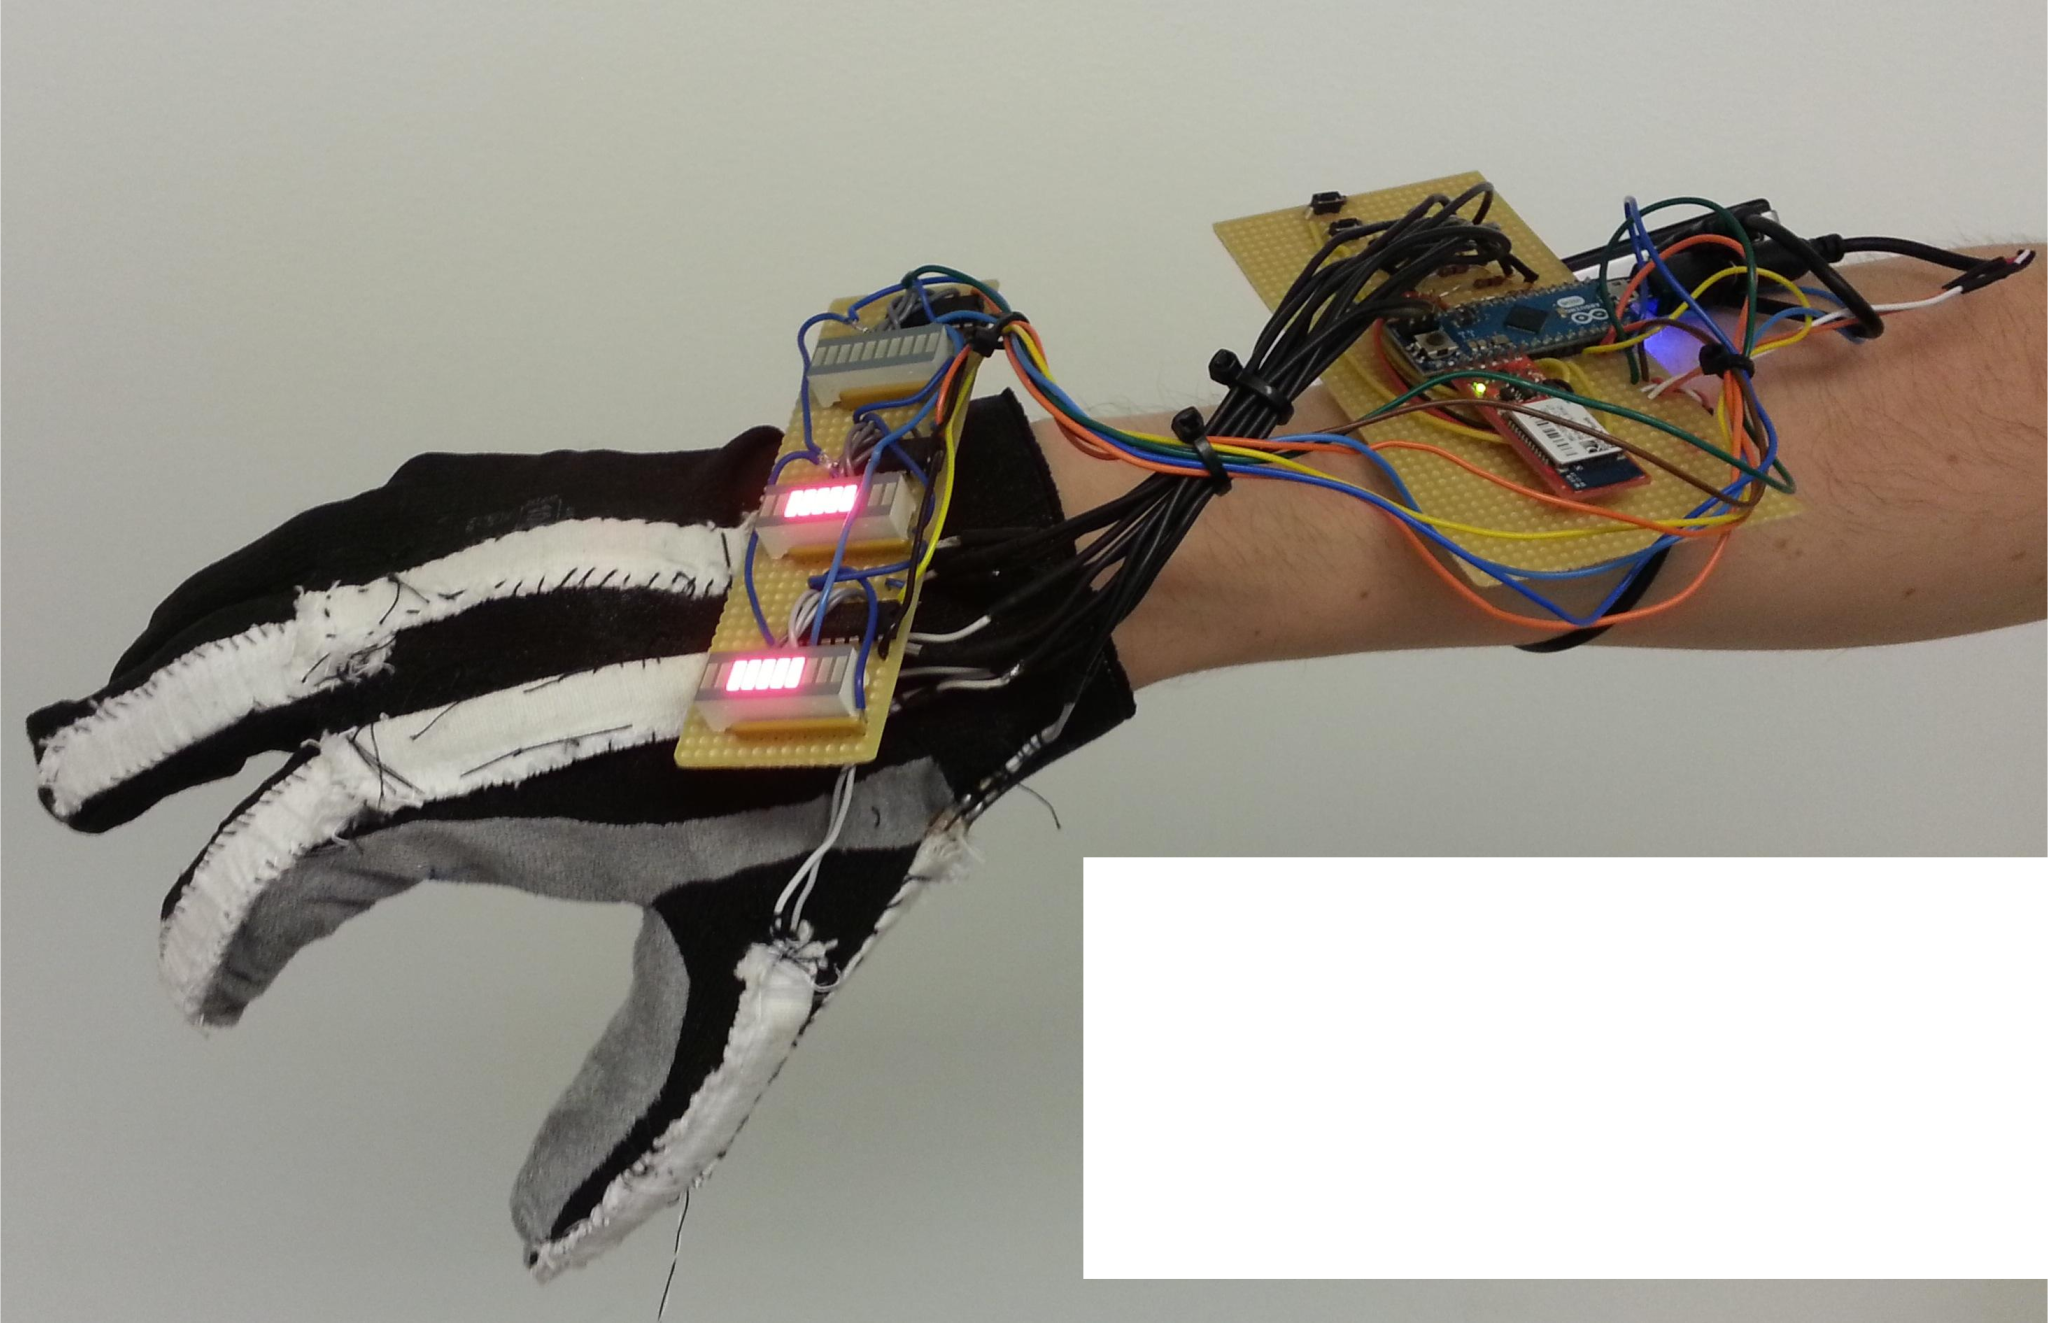
\includegraphics[width=\textwidth]{img/styrhandskediod}
\end{frame}

\section{Signalbehandling}

\begin{frame}
\frametitle{Signalens väg för robothanden}
\begin{tikzpicture}[node distance = 3.5cm, auto]
    \node [block] (sampling) {trycksensorernas spänning samplas};
    \node [block, right of=sampling] (filter) {störningar filtreras};
    \node [block, right of=filter] (norm1) {spänningen tolkas som en relativ kraft};

    \path [line] (sampling) -- (filter);
    \path [line] (filter) -- (norm1);
 \end{tikzpicture}
\end{frame}


\begin{frame}
\centering
\begin{tikzpicture}[node distance = 3.5cm, auto]
% \vspace*{\fill}
\scriptsize
    \node [block] (sampling) {trycksensorernas spänning samplas};
    \node [blockfat, right of=sampling] (filter) {störningar filtreras};
    \node [block, right of=filter] (norm1) {spänningen tolkas som en relativ kraft};

    \path [line] (sampling) -- (filter);
    \path [line] (filter) -- (norm1);
\end{tikzpicture}

\includegraphics[width=\textwidth]{img/tryck_dubbel.pdf}
\scriptsize
\[
G(s) = \frac{\omega_0}{\omega_0 + s},\omega_0 = 2\pi f_0\;\; \Rightarrow \;\;
y[n] = \frac{f_0(x[n]+x[n-1]) - y[n-1](f_0 - 2f_s)}{f_0 + 2f_s}
\]
\end{frame}



\begin{frame}
\centering
\begin{tikzpicture}[node distance = 3.5cm, auto]
\scriptsize
    \node [block] (sampling) {trycksensorernas spänning samplas};
    \node [block, right of=sampling] (filter) {störningar filtreras};
    \node [blockfat, right of=filter] (norm1) {spänningen tolkas som en relativ kraft};

    \path [line] (sampling) -- (filter);
    \path [line] (filter) -- (norm1);
\end{tikzpicture}
\vspace*{\fill}
\begin{columns}
\begin{column}[t]{0.5\textwidth}
\includegraphics[width=\textwidth]{img/before.pdf}
\[
    f(x) = a\left(1-e^{-x/b}\right) x^d
\]
\end{column}
\begin{column}[t]{0.5\textwidth}
\includegraphics[width=\textwidth]{img/after.pdf}
\[ f^{-1}(x) = \text{interpolering}
\]
\end{column}
\end{columns}

\end{frame}



\begin{frame}
\frametitle{Signalens väg för styrhandsken}
\footnotesize
\begin{tikzpicture}[node distance = 2.8cm, auto]
    \node [blockfade] (sampling) {flexsensorernas spänning samplas};
    \node [blockfade, right of=sampling] (filter) {störningar filtreras};
    \node [block, right of=filter] (norm1) {normalisering mot användarens hand};
    \node [block, right of=norm1] (norm2) {normalisering mot robothandens vinklar};

    \path [line] (sampling) -- (filter);
    \path [line] (filter) -- (norm1);
    \path [line] (norm1) -- (norm2);
\end{tikzpicture}
\begin{itemize}
    \item De två första stegen som för robothanden
\end{itemize}
\end{frame}



\section{Objektidentifiering}
\begin{frame}
\frametitle{Servovinklar}
\includegraphics[width=\textwidth]{img/servo_vinklar}
\end{frame}

\begin{frame}
\frametitle{Identifiering}
\begin{center}
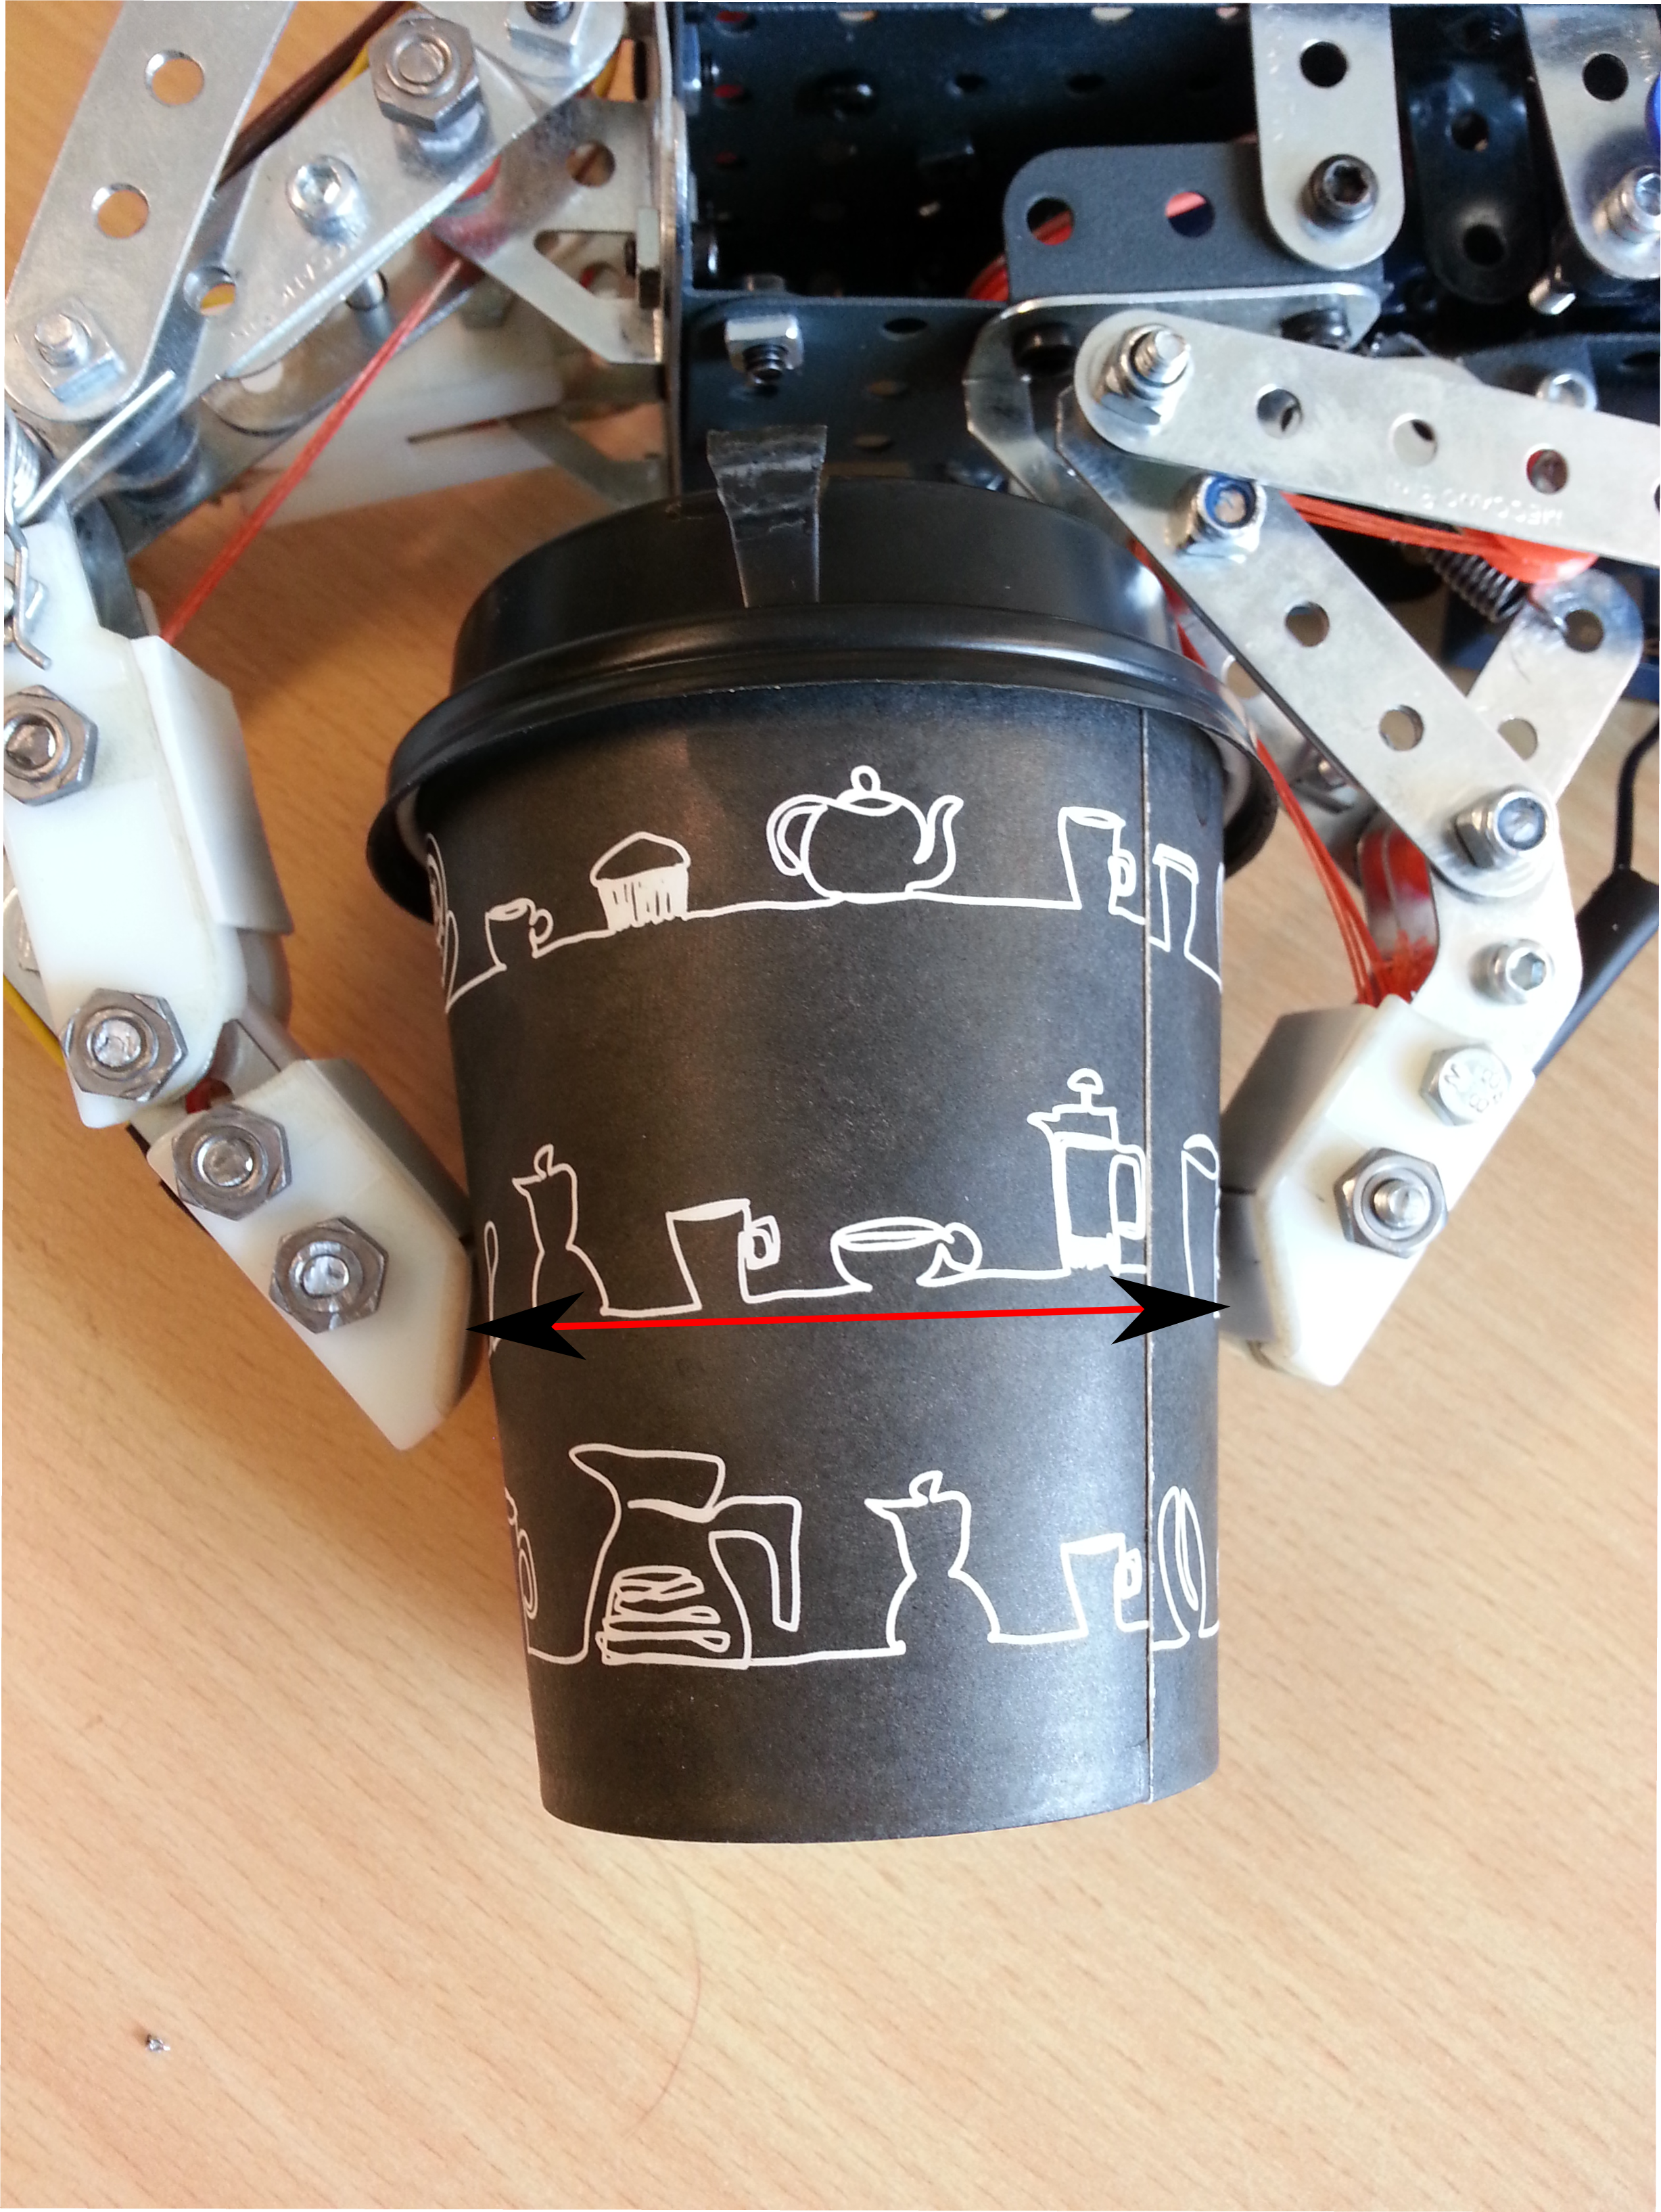
\includegraphics[width=0.5\textwidth]{img/obj_dist}
\end{center}
\end{frame}

\begin{frame}
\frametitle{Modell av handen}
\includegraphics[width=\textwidth]{img/matlab_modell}
\end{frame}

\begin{frame}
\frametitle{Jämförelse mot verkliga värden}
\includegraphics[width=\textwidth]{img/obj_id_matlab2-eps-converted-to}
\end{frame}

\section{Tryckbegränsning}
\begin{frame}
\frametitle{Tryckbegränsning}
\includegraphics[width=\textwidth]{img/masterplot}
\end{frame}

\section{Reflektioner}
\begin{frame}
\frametitle{Reflektioner}
\begin{columns}
\begin{column}[t]{0.5\textwidth}
\textbf{Bra}
\begin{itemize}
    \item Intuitiv styrning
    \item Användarvänlig
    \item Klarar av flera grepp
    \item Kraftåterkoppling
\end{itemize}
\end{column}
\begin{column}[t]{0.5\textwidth}
\textbf{Kan förbättras}
\begin{itemize}
	\item Meccano
	\item Återkoppling av vinklar
	\item Vikten av bra sensorer
	\item Latenstider (bluetooth inte optimalt)
\end{itemize}
\end{column}
\end{columns}
\end{frame}
